\subsection{Introduction}

\begin{frame}{Bootloader role}
  \begin{itemize}
  \item The bootloader is a piece of code responsible for
    \begin{itemize}
    \item Basic hardware initialization
    \item Loading of an application binary, usually an operating
      system kernel, from flash storage, from the network, or from
      another type of non-volatile storage.
    \item Possibly decompression of the application binary
    \item Execution of the application
    \end{itemize}
  \item Besides these basic functions, most bootloaders provide a
    shell or menu
    \begin{itemize}
    \item Menu to select the operating system to load
    \item Shell with commands to load data from storage or network,
      inspect memory, perform hardware testing/diagnostics
    \end{itemize}
  \item The first piece of code running by the processor that can be
    modified by us developers.
  \end{itemize}
\end{frame}

\subsection{Booting on x86 platforms}

\begin{frame}{Legacy BIOS booting (1)}
  \begin{itemize}
  \item x86 platforms shipped before 2005-2006 include a firmware
    called {\em BIOS}
    \begin{itemize}
    \item BIOS = Basic Input Output System
    \item Part of the hardware platform, closed-source, rarely
      modifiable
    \item Implements the booting process
    \item Provides runtime services that can be invoked - not commonly
      used
    \item Stored in some flash memory, outside of regular
      user-accessible storage devices
    \end{itemize}
  \item To be bootable, the first sector of a storage device is
    ``special''
    \begin{itemize}
    \item MBR = Master Boot Record
    \item Contains the partition table
    \item Contains up to 446 bytes of bootloader code, loaded into RAM
      and executed
    \item The BIOS is responsible for the RAM initialization
    \end{itemize}
  \item \url{https://en.wikipedia.org/wiki/BIOS}
  \end{itemize}
\end{frame}

\begin{frame}{Legacy BIOS booting (2)}
  \begin{itemize}
  \item Due to the limitation in size of the bootloader, bootloaders
    are split into two stages
    \begin{itemize}
    \item Stage 1, which fits within the 446 bytes constraint
    \item Stage 2, which is loaded by stage 1, and can therefore be
      bigger
    \end{itemize}
  \item Stage 2 is typically stored outside of any filesystem, at a
    fixed offset $\rightarrow$ simpler to load by stage 1
  \item Stage 2 generally has filesystem support, so it can load the
    kernel image from a filesystem
  \end{itemize}
\end{frame}

\begin{frame}{Legacy BIOS booting: sequence and storage}
  \begin{center}
    \includegraphics[width=0.7\textwidth]{slides/sysdev-bootloaders-sequence/legacy-bios-sequence.pdf}\\
    \vspace{0.5cm}
    \includegraphics[width=0.9\textwidth]{slides/sysdev-bootloaders-sequence/legacy-bios-storage.pdf}
  \end{center}
\end{frame}

\begin{frame}{UEFI booting}
  \begin{itemize}
  \item Starting from 2005-2006, UEFI is the new firmware interface on
    x86 platforms
    \begin{itemize}
    \item Unified Extensible Firmware Interface
    \item Describes the interface between the operating system and the
      firmware
    \item Firmware in charge of booting
    \item Firmware also provides runtime services to the operating
      system
    \item Stored in some flash memory, outside of regular
      user-accessible storage devices
    \end{itemize}
  \item Loads EFI binaries from the {\em EFI System Partition}
    \begin{itemize}
    \item Generally a bootloader
    \item Can also be directly the Linux kernel, with an {\em EFI Boot
        Stub}
    \end{itemize}
  \item Special partition, formatted with the {\em FAT} filesystem
    \begin{itemize}
    \item MBR: identified by type \code{0xEF}
    \item GPT: identified with a specific {\em globally unique identifier}
    \end{itemize}
  \item File \code{/efi/boot/bootx32.efi}, \code{/efi/boot/bootx64.efi}
  \item \url{https://en.wikipedia.org/wiki/UEFI}
  \end{itemize}
\end{frame}

\begin{frame}{UEFI booting: sequence and storage}
  \begin{center}
    \vspace{0.5cm}
    \includegraphics[width=0.7\textwidth]{slides/sysdev-bootloaders-sequence/uefi-sequence.pdf}\\
    \vspace{0.5cm}
    \includegraphics[width=0.9\textwidth]{slides/sysdev-bootloaders-sequence/uefi-storage.pdf}\\
  \end{center}
\end{frame}

\begin{frame}{ACPI}
  \begin{itemize}
  \item Advanced Configuration and Power Interface
  \item {\em Open standard that operating systems can use to discover
      and configure computer hardware components, to perform power
      management, to perform auto configuration, and to perform status
      monitoring}
  \item {\em Tables} with descriptions of the hardware that cannot be
    dynamically discovered at runtime
  \item Tables provided by the firmware (UEFI or legacy) and used by
    the operating system (Linux kernel in our case)
  \item \small \url{https://en.wikipedia.org/wiki/Advanced_Configuration_and_Power_Interface}
  \end{itemize}
\end{frame}

\begin{frame}{UEFI and ACPI on ARM}
  \begin{itemize}
  \item Historically UEFI and ACPI are technologies coming from the
    Intel/x86 world
  \item ARM is also pushing for the adoption of UEFI and ACPI as part
    of its {\em ARM System Ready} certification
    \begin{itemize}
    \item Mainly for servers/workstations SoCs
    \item Does not impact embedded SoCs
    \item Currently not common in embedded Linux projects on ARM
    \item \url{https://www.arm.com/architecture/system-architectures/systemready-certification-program}
    \end{itemize}
  \item Also some on-going effort to use UEFI on RISC-V, but not the
    de-facto standard
  \item When an embedded platform uses UEFI $\rightarrow$ its booting
    process is similar to an {\em x86} platform
  \end{itemize}
\end{frame}

\subsection{Booting on embedded platforms}

\begin{frame}{Booting on embedded platforms: ROM code}
  \begin{itemize}
  \item Most embedded processors include a {\bf ROM code} that
    implements the initial step of the boot process
  \item The ROM code is written by the processor vendor and directly
    built into the processor
    \begin{itemize}
    \item Cannot be changed or updated
    \item Its behavior is described in the processor datasheet
    \end{itemize}
  \item Responsible for finding a suitable bootloader, loading it and
    running it
    \begin{itemize}
    \item From NAND/NOR flash, from USB, from SD card, from eMMC, etc.
    \item Well defined location/format
    \end{itemize}
  \item {\em Generally} runs with the external RAM not initialized, so
    it can only load the bootloader into an internal SRAM
    \begin{itemize}
    \item Limited size of the bootloader, due to the size of the SRAM
    \item Forces the boot process to be split in two steps: first
      stage bootloader (small, runs from SRAM, initializes external DRAM),
      second stage bootloader (larger, runs from external DRAM)
    \end{itemize}
  \end{itemize}
\end{frame}

\begin{frame}{Booting on STM32MP1: datasheet}
  \begin{columns}
    \column{0.7\textwidth}
    \begin{center}
      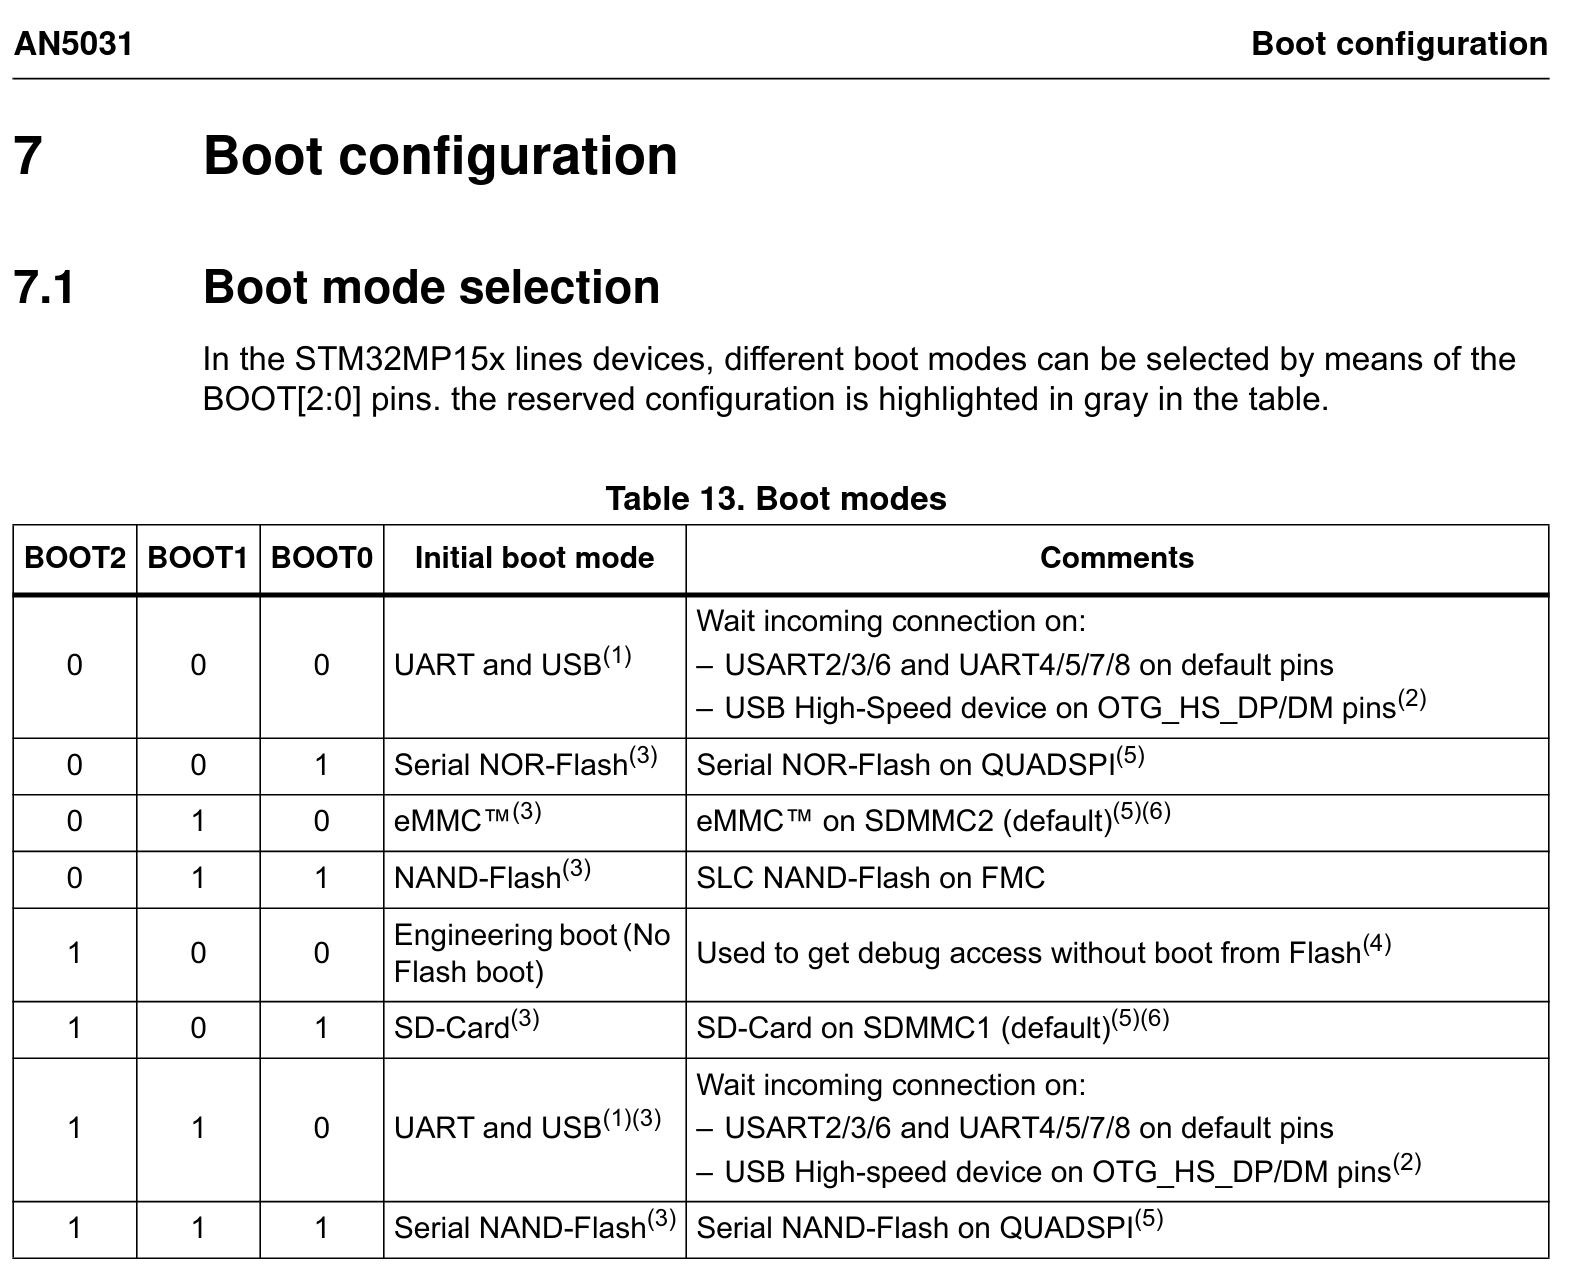
\includegraphics[height=0.85\textheight]{slides/sysdev-bootloaders-sequence/stm32mp1-rom-code.png}
    \end{center}
    \column{0.3\textwidth}
    {\tiny
      Source: \url{https://www.st.com/resource/en/application_note/dm00389996-getting-started-with-stm32mp151-stm32mp153-and-stm32mp157-line-hardware-development-stmicroelectronics.pdf}\\
      Useful details: \url{https://wiki.st.com/stm32mpu/wiki/STM32_MPU_ROM_code_overview}
    }
  \end{columns}
\end{frame}

\begin{frame}{Booting on AM335x: datasheet}
  \begin{columns}
      \column{0.6\textwidth}
      \begin{center}
        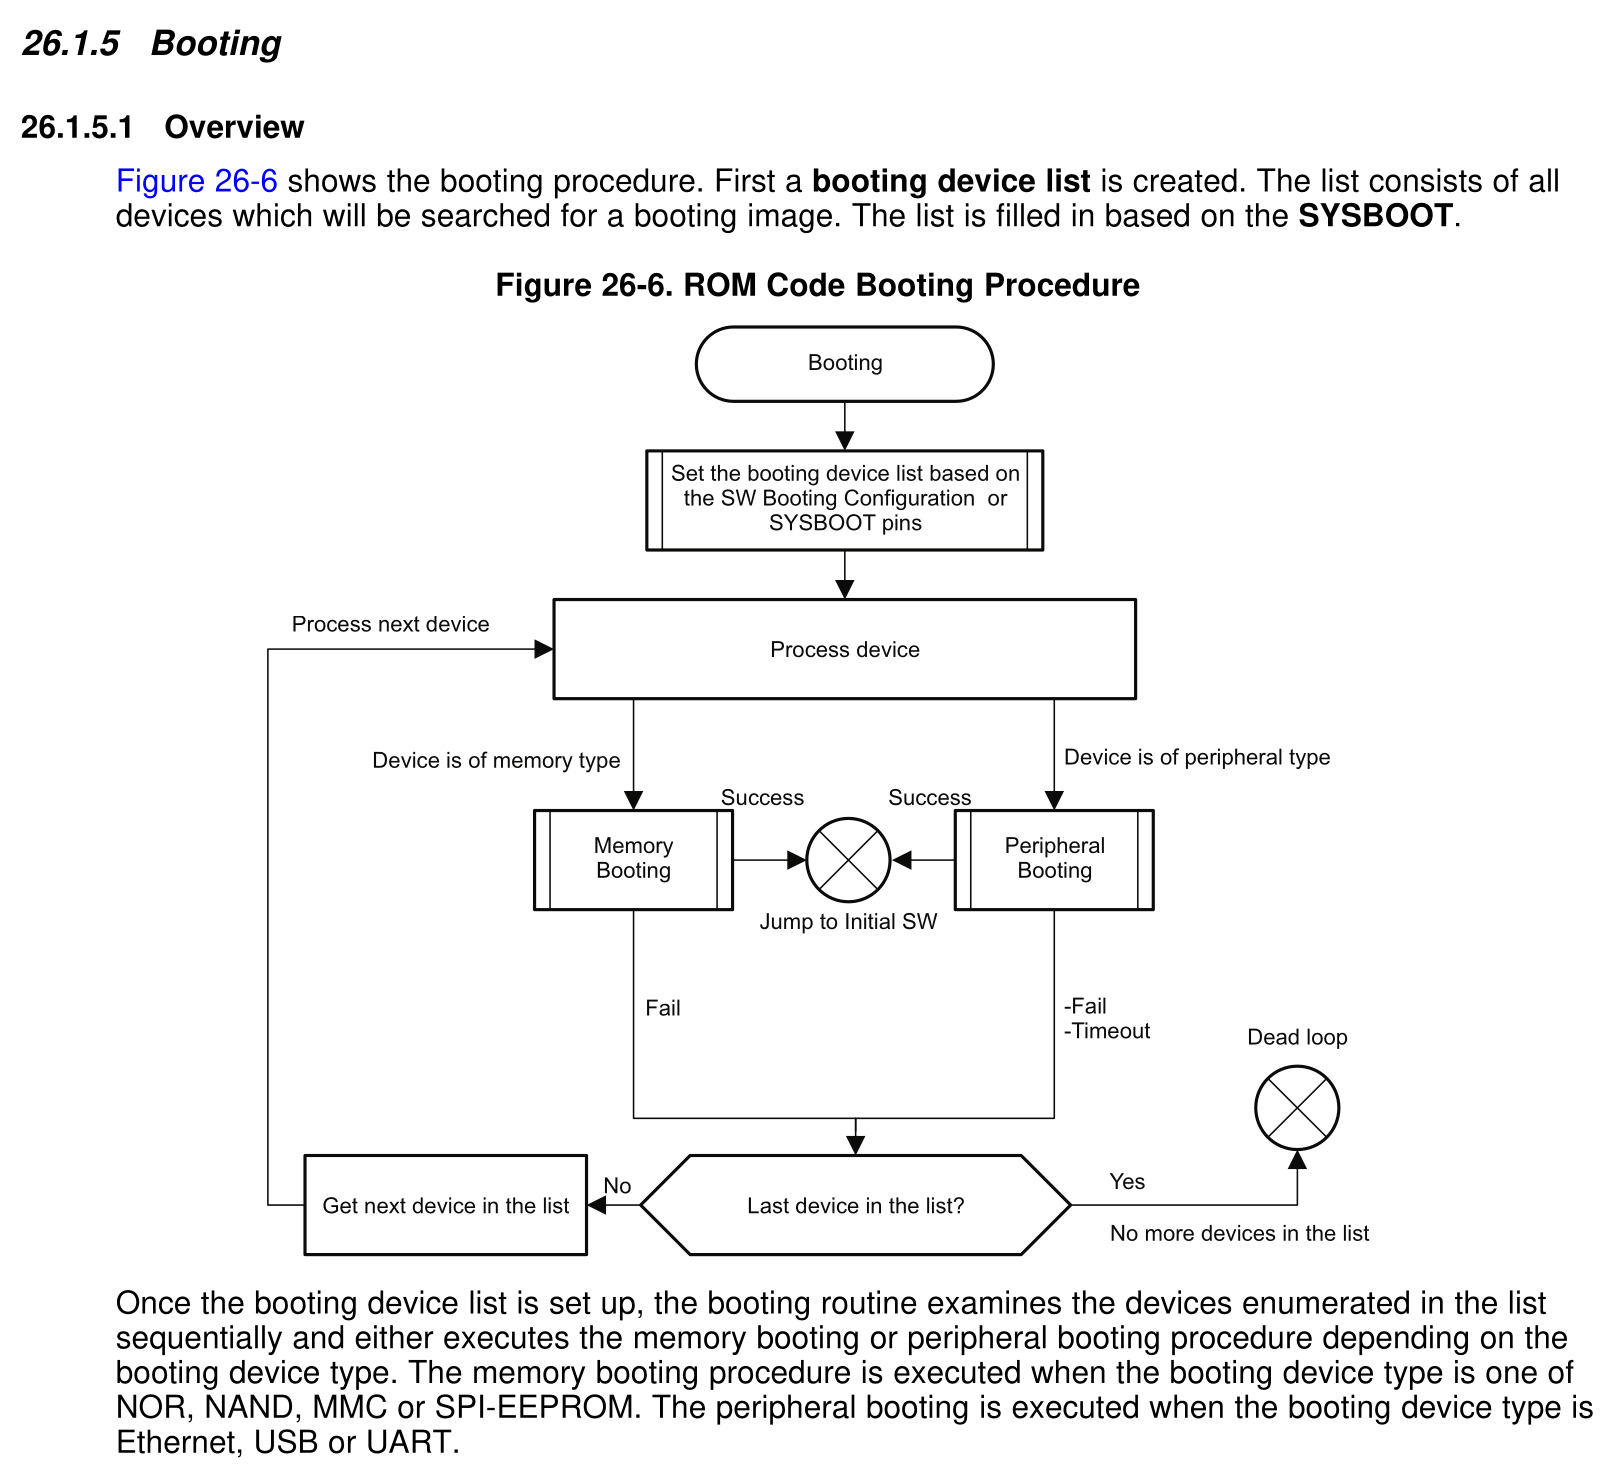
\includegraphics[height=0.85\textheight]{slides/sysdev-bootloaders-sequence/am335x-rom-code.png}
      \end{center}
      \column{0.4\textwidth}
      {\tiny
        Source:\\
        \url{https://www.mouser.com/pdfdocs/spruh73h.pdf},\\
	chapter 26
      }
    \end{columns}
\end{frame}

\begin{frame}{Two stage booting sequence}
  \begin{center}
    \includegraphics[height=0.85\textheight]{slides/sysdev-bootloaders-sequence/two-step-boot-process.pdf}
  \end{center}
\end{frame}

\begin{frame}{ROM code recovery mechanism}
  \begin{columns}
    \column{0.6\textwidth}
    \begin{itemize}
    \item Most ROM code also provide some sort of {\em recovery}
      mechanism
    \item Allows to flash a board with no bootloader or a broken
      bootloader
    \item Typically using a vendor-specific protocol over UART or USB
    \item Often allows to push a new bootloader into memory, thanks to
      which reflashing a working bootloader is possible
    \item Vendor-specific tool to run on the workstation
      \begin{itemize}
      \item STM32MP1: \href{https://www.st.com/en/development-tools/stm32cubeprog.html}{STM32 Cube Programmer}
      \item NXP i.MX: \href{https://github.com/NXPmicro/mfgtools}{uuu}
      \item Microchip AT91/SAM: \href{https://www.microchip.com/en-us/development-tool/SAM-BA-In-system-Programmer}{SAM-BA}
      \item Allwinner: \href{https://github.com/linux-sunxi/sunxi-tools}{sunxi-fel}
      \item Some open-source, some proprietary
      \end{itemize}
    \end{itemize}
    \column{0.4\textwidth}
    \includegraphics[width=\textwidth]{slides/sysdev-bootloaders-sequence/stm32mp1-rom-code-recovery.pdf}
  \end{columns}
\end{frame}

\subsection{Bootloaders}

\begin{frame}{GRUB}
  \begin{columns}
    \column{0.6\textwidth}
    \begin{itemize}
    \item {\em Grand Unified Bootloader}, from the GNU project
    \item De-facto standard in most Linux distributions for x86
      platforms
    \item Supports x86 legacy and UEFI systems
    \item Can read many filesystem formats to load the kernel image,
      modules and configuration
    \item Provides a menu and powerful shell with various commands
    \item Can load kernel images over the network
    \item Also supports ARM, ARM64, RISC-V, PowerPC, but less popular
      than other bootloaders on those platforms
    \item \url{https://www.gnu.org/software/grub/}
    \item \url{https://en.wikipedia.org/wiki/GNU_GRUB}
    \end{itemize}
    \column{0.4\textwidth}
    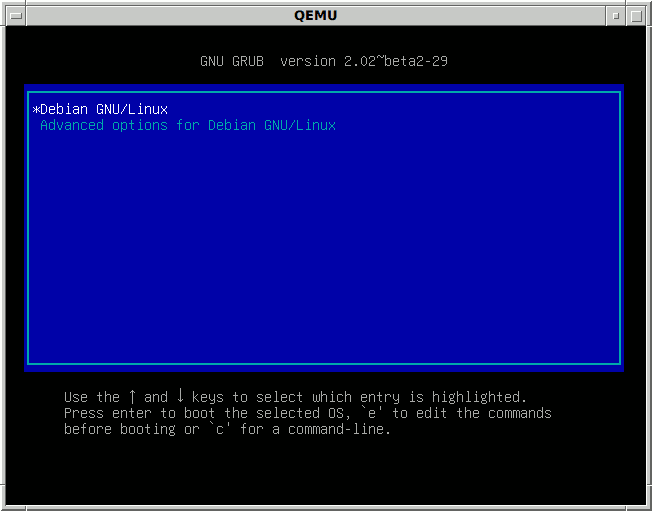
\includegraphics[width=\textwidth]{slides/sysdev-bootloaders-sequence/grub2.png}
  \end{columns}
\end{frame}

\begin{frame}{Syslinux}
  \begin{columns}
    \column{0.8\textwidth}
    \begin{itemize}
    \item For network and removable media booting (USB key, SD card, CD-ROM)
    \item \code{syslinux}: booting from FAT filesystem
    \item \code{pxelinux}: booting from the network
    \item \code{isolinux}: booting from CD-ROM
    \item \code{extlinux}: booting from numerous filesystem types
    \item A bit rustic to build and configure, not very actively
      maintained, but still useful for specific use-cases
    \item \url{https://wiki.syslinux.org/}
    \item \url{https://kernel.org/pub/linux/utils/boot/syslinux/}
    \end{itemize}
    \column{0.2\textwidth}
    
\includegraphics[width=\textwidth]{slides/sysdev-bootloaders-sequence/syslinux.png}
  \end{columns}
\end{frame}

\begin{frame}{systemd-boot}
  \begin{columns}
    \column{0.7\textwidth}
    \begin{itemize}
    \item Simple UEFI boot manager
    \item Useful alternative to GRUB for UEFI systems: simpler than GRUB
    \item Configured using files stored in the {\em EFI System
        Partition}
    \item Part of the {\em systemd} project, even though obviously
      distinct from {\em systemd} itself
      \begin{itemize}
      \item See our slides later in this course for more details on {\em
          systemd}
      \end{itemize}
    \item \url{https://www.freedesktop.org/wiki/Software/systemd/systemd-boot/}
    \end{itemize}
    \column{0.3\textwidth}
    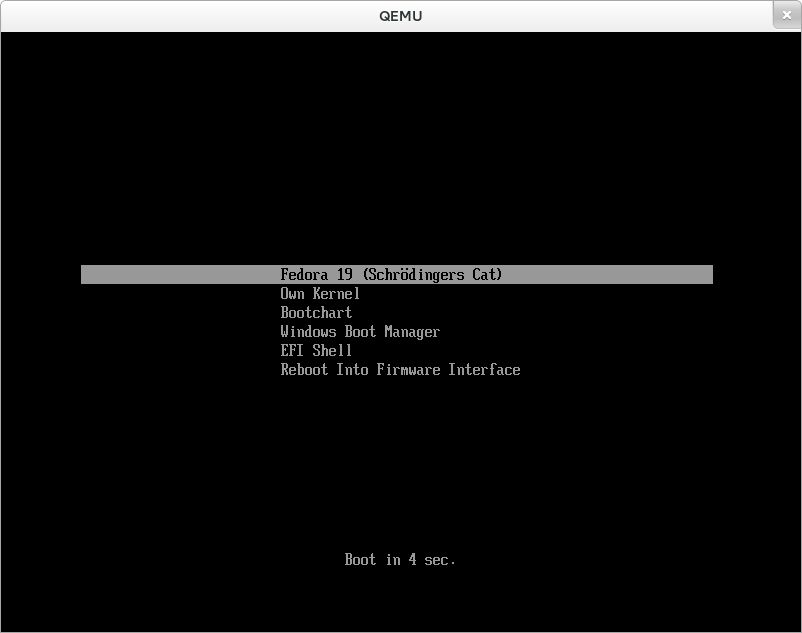
\includegraphics[width=\textwidth]{slides/sysdev-bootloaders-sequence/systemd-boot.png}
  \end{columns}
\end{frame}

\begin{frame}{shim}
  \begin{itemize}
  \item Minimal UEFI bootloader
  \item Mainly used in secure boot scenario: it is signed by Microsoft
    and therefore successfully verified by UEFI firmware in the field
  \item Allows to chainload another bootloader (GRUB) or directly
    the Linux kernel, with signature checking
  \item \url{https://github.com/rhboot/shim}
  \end{itemize}
\end{frame}

\begin{frame}{U-Boot}
  \begin{columns}
    \column{0.7\textwidth}
    \begin{itemize}
    \item The de-facto standard and most widely used bootloader on
      embedded architectures: ARM, ARM64, RISC-V, PowerPC, MIPS, and
      more.
    \item Also supports x86 with UEFI firmware.
    \item Very likely the one provided by your SoC vendor, SoM vendor
      or board vendor for your hardware.
    \item We will study it in detail in the next section, and use it in
      all practical labs of this course.
    \item \url{https://www.denx.de/wiki/U-Boot}
    \end{itemize}
    \column{0.3\textwidth}
    
\includegraphics[width=\textwidth]{slides/sysdev-bootloaders-sequence/u-boot.png}
  \end{columns}
\end{frame}

\begin{frame}{Barebox}
  \begin{columns}
    \column{0.7\textwidth}
    \begin{itemize}
    \item Another bootloader for most embedded CPU architectures:
      ARM/ARM64, MIPS, PowerPC, RISC-V, x86, etc.
    \item Initially developed as an alternative to U-Boot to address
      some U-Boot shortcomings
      \begin{itemize}
      \item {\em kconfig} for the configuration like the Linux kernel
      \item well-defined {\em device model} internally
      \item More Linux-style shell interface
      \item Cleaner code base
      \end{itemize}
    \item Actively maintained and developed, but
      \begin{itemize}
      \item Less widely used than U-Boot
      \item Less platform support than in U-Boot
      \end{itemize}
    \item \url{https://www.barebox.org/}
    \item Talk {\em barebox Bells and Whistles}, by Ahmad Fatoum, ELCE
      2020, \href{https://youtu.be/Oj7lKbFtyM0}{video} and
      \href{https://elinux.org/images/9/9d/Barebox-bells-n-whistles.pdf}{slides}
    \end{itemize}
    \column{0.3\textwidth}
    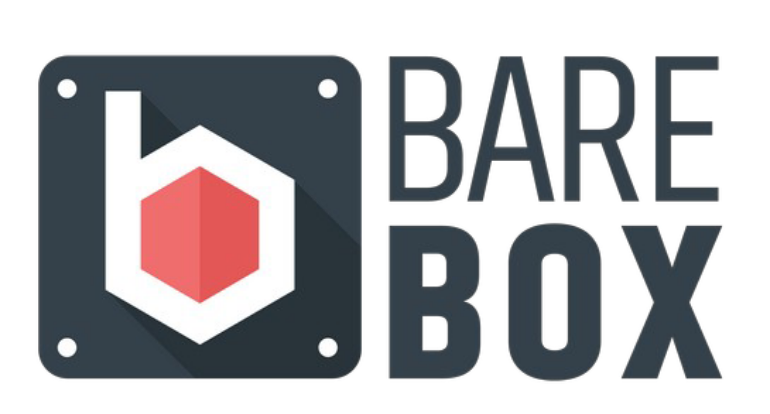
\includegraphics[width=\textwidth]{slides/sysdev-bootloaders-sequence/barebox.png}
  \end{columns}
\end{frame}

\subsection{Trusted firmware}

\begin{frame}{Concept}
  \begin{itemize}
  \item Traditionally, bootloaders are only used during the booting
    process
    \begin{itemize}
    \item Bootloader loads operating system, jumps to it, and is
      discarded
    \end{itemize}
  \item Modern SoCs have advanced security mechanisms that require
    running some sort of {\em trusted firmware}
  \item This firmware is loaded by the bootloader, or part of the boot
    chain itself
  \item This {\em trusted firmware} {\bf stays resident} after control
    has been passed to the OS
    \begin{itemize}
    \item It is stored in a dedicated portion of the DDR, or some
      specific SRAM, inaccessible from the OS
    \item It provides services to the OS, which the OS cannot perform
      directly
    \item Can also be responsible for running a secure OS alongside the
      regular OS (Linux in our case)
    \end{itemize}
  \end{itemize}
\end{frame}

\begin{frame}{ARM}
  \begin{itemize}
  \item Modern ARMv7 and ARMv8 processors have
    \begin{itemize}
    \item 4 privilege levels ({\em Exception Levels})
      \begin{itemize}
      \item EL3, the most priviledged, runs secure firmware
      \item EL2, typically used by hypervisors, for virtualization
      \item EL1, used to run the Linux kernel
      \item EL0, used to run Linux user-space applications
      \end{itemize}
    \item 2 {\em worlds}
      \begin{itemize}
      \item Normal world, used to run a general purpose OS, like Linux
      \item Secure world, to run a separate, isolated, secure
        operating system and applications. Also called {\em TrustZone}
        by ARM.
      \end{itemize}
    \end{itemize}
  \item EL3 only exists in the secure world
  \item EL2 exists in both secure and normal worlds since ARMv8.4,
    before that EL2 was only in the normal world
  \item EL1 and EL0 exist in both secure and normal worlds
  \end{itemize}
\end{frame}

\begin{frame}{ARM exception levels and worlds}
  \begin{center}
    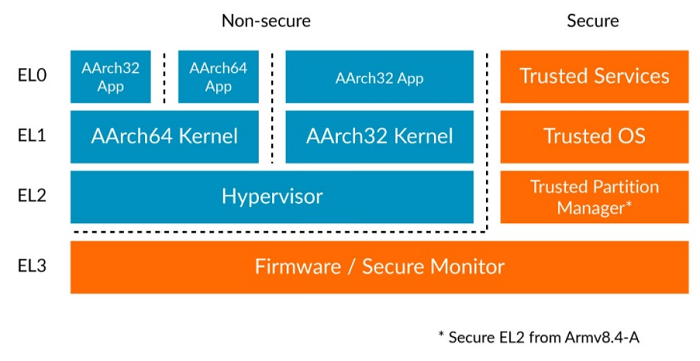
\includegraphics[height=0.75\textheight]{slides/sysdev-bootloaders-sequence/arm-exception-levels.png}
  \end{center}
  Source: \href{https://developer.arm.com/documentation/102412/0102/Execution-and-Security-states}{ARM documentation}
\end{frame}

\begin{frame}{Interfaces with secure firmware}
  \begin{columns}
    \column{0.8\textwidth}
    \begin{itemize}
    \item Standardized by ARM
    \item Services
      \begin{itemize}
      \item implemented by the secure firmware
      \item called by the operating system
      \end{itemize}
    \item Prevents the operating system running in normal world from
      directly accessing critical hardware resources
    \item
      \href{http://infocenter.arm.com/help/topic/com.arm.doc.den0022d/Power_State_Coordination_Interface_PDD_v1_1_DEN0022D.pdf}{PSCI},
      Power State Coordination Interface
      \begin{itemize}
      \item Power management related: turn CPUs on/off, CPU idle state,
        platform shutdown/reset
      \end{itemize}
    \item
      \href{http://infocenter.arm.com/help/topic/com.arm.doc.den0056a/DEN0056A_System_Control_and_Management_Interface.pdf}{SCMI},
      System Control and Management Interface
      \begin{itemize}
      \item Power domain, clocks, sensor, performance
      \end{itemize}
    \item Secure firmware implementing these interfaces is
      \begin{itemize}
      \item Mandatory to run Linux on ARMv8
      \item Mandatory to run Linux on some ARMv7 platforms, but not all
      \end{itemize}
    \end{itemize}
    \column{0.2\textwidth}
    \includegraphics[width=\textwidth]{slides/sysdev-bootloaders-sequence/arm-interfaces.pdf}
  \end{columns}
\end{frame}

\begin{frame}{TF-A}
  \begin{itemize}
  \item {\em Trusted Firmware-A (TF-A) provides a reference
      implementation of secure world software for Armv7-A and Armv8-A,
      including a Secure Monitor executing at Exception Level 3 (EL3)}
  \item Formerly known as {\em ATF}, for ARM Trusted Firmware
  \item Implements the various standard interfaces that operating
    systems need from the secure firmware
  \item Has drivers for the hardware blocks that are not accessed
    directly by Linux
  \item Needs to be ported for each SoC
  \item Depending on the platform, may also need to be ported per
    board: DDR initialization
  \item Used on the vast majority of ARMv8 platforms, and on a few
    recent ARMv7 platforms
  \item \url{https://www.trustedfirmware.org/projects/tf-a/}
  \end{itemize}
\end{frame}

\begin{frame}{Trusted OS, OP-TEE}
  \begin{itemize}
  \item A trusted operating system can run in the {\em secure world},
    also called {\em Trusted Execution Environment} or {\em TEE}
  \item Hardware partitioning between {\em secure world} and {\em
      normal world}
    \begin{itemize}
    \item Some hardware resources only available in the {\em secure
        world}, by the trusted OS
    \end{itemize}
  \item Allows to run trusted applications/services
    \begin{itemize}
    \item isolated from Linux
    \item can provide services to Linux applications
    \end{itemize}
  \item Most common open-source implementation: {\em OP-TEE}
    \begin{itemize}
    \item Supported by most silicon vendors
    \item \url{https://www.op-tee.org/}
    \end{itemize}
  \end{itemize}
\end{frame}

\begin{frame}{ARM: summary}
  \begin{center}
    \includegraphics[height=0.70\textheight]{slides/sysdev-bootloaders-sequence/arm-nomenclature.pdf}
  \end{center}
  {\small Largely inspired from {\em Ahmad Fatoum} presentation
    {\em From Reset Vector to Kernel},
    \href{https://archive.fosdem.org/2021/schedule/event/from_reset_vector_to_kernel/attachments/slides/4632/export/events/attachments/from_reset_vector_to_kernel/slides/4632/from_reset_vector_to_kernel.pdf}{slides},
    \href{https://www.youtube.com/watch?v=-Ak9MWGxd7M}{video}}\\
    See also
    \href{https://trustedfirmware-a.readthedocs.io/en/latest/design/firmware-design.html}
    {details about the ARM terms: BL1, BL2...}
\end{frame}

\begin{frame}{RISC-V}
  \begin{columns}
    \column{0.7\textwidth}
    \begin{itemize}
    \item Linux-class RISC-V processors have several privilege levels
      \begin{itemize}
      \item M-mode: machine mode
      \item S-mode: level at which the Linux kernel runs
      \item U-mode: level at which Linux user-space
        applications run
      \end{itemize}
    \item Some specific HW resources are not accessible in S-mode
    \item A more priviledged firmware runs in M-mode
    \item RISC-V has defined SBI, {\em Supervisor Binary Interface}
      \begin{itemize}
      \item Standardized interface between the OS and the firmware
      \item \url{https://github.com/riscv-non-isa/riscv-sbi-doc}
      \end{itemize}
    \item OpenSBI is a reference, open-source implementation of SBI
      \begin{itemize}
      \item \url{https://github.com/riscv-software-src/opensbi}
      \end{itemize}
    \end{itemize}
    \column{0.3\textwidth}
    \includegraphics[width=\textwidth]{slides/sysdev-bootloaders-sequence/riscv-boot.pdf}
  \end{columns}
\end{frame}

\subsection{Example boot sequences on ARM}

\begin{frame}{TI AM335x: ARMv7}
  \begin{center}
    \includegraphics[width=\textwidth]{slides/sysdev-bootloaders-sequence/sequence-am335x.pdf}
  \end{center}
\end{frame}

\begin{frame}{NXP i.MX6: ARMv7}
  \begin{center}
    \includegraphics[height=0.7\textheight]{slides/sysdev-bootloaders-sequence/sequence-imx.pdf}
  \end{center}
  \vspace{0.1cm}
  Note: this diagram shows one possible boot flow on NXP i.MX6, but it
  is also possible to use the U-Boot SPL $\rightarrow$ U-Boot boot
  flow on i.MX6.
\end{frame}

\begin{frame}{STM32MP1: ARMv7}
  \begin{center}
    \includegraphics[width=\textwidth]{common/sequence-stm32mp1.pdf}
  \end{center}
  \vspace{0.3cm}
  Note: booting with U-Boot SPL and U-Boot is also possible.
\end{frame}

\begin{frame}{Allwinner ARMv8 cores}
  \begin{center}
    \includegraphics[height=0.8\textheight]{slides/sysdev-bootloaders-sequence/sequence-allwinner-64-bit.pdf}
  \end{center}
\end{frame}
